\chapter{Обзор существующих решений} \label{ch2}
В данной главе будут рассмотрены существующие средства визуализации, определены их плюсы и минусы и указан краткий обзор.
\section{Анализ существующих средств визуализации моделей программ} \label{ch2:sec1}
Существует множество вариантов архитектуры визуализатора. Это может быть как десктопное приложение, как мобильное, как клиент-серверное. Для анализа были выбраны визуализаторы, находящиеся в свободном доступе и максимально приближенные к желаемому результату.
\section{Анализ существующих средств визуализации моделей программ} \label{ch2:sec1-abbr}
ANTLR (Another Tool for Language Recognition) – это мощный генератор парсеров. С его помощью можно сгенерировать парсер для любой заданной грамматики, в том числе для языков программирования. Для генерации парсера нужен файл грамматики, составленный по определённым правилам. Существует множество готовых грамматик для разных языков, в том числе для языка программирования Java. Кроме того, есть возможность вывести дерево парсинга в графическом интерфейсе.
Сам по себе ANTLR не является готовым решением для построения и визуализации AST. Он лишь может сгенерировать код по шаблону (Visitor или Listener) на одном из поддерживаемых языков программирования, который можно дописать для получения желаемого результата. Дерево парсинга, которое получается при использовании ANTLR, содержит в себе все символы исходного текста. Чтобы из этого построить AST, необходимо убрать множество лишних элементов.
\begin{figure}[ht!] 
	\center
	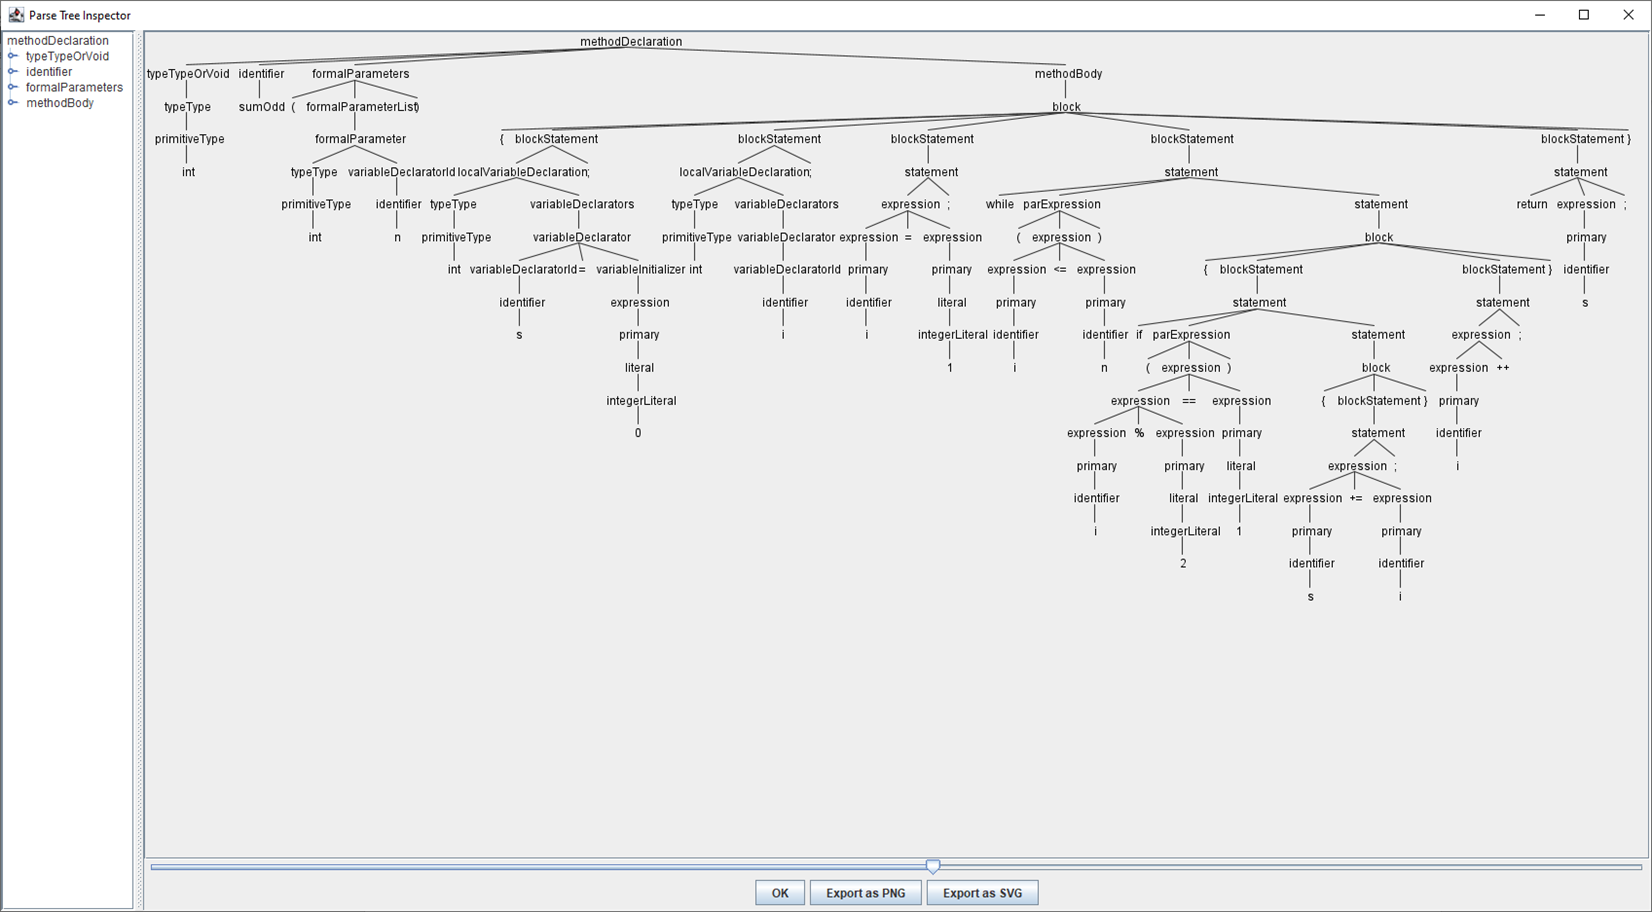
\includegraphics [scale=0.27] {my_folder/images/my/8}
	\caption{Графический интерфейс ANTLR} 
	\label{fig:8}  
\end{figure}
\subsection{AST Explorer} \label{ch2:subsec-title-abbr}
AST Explorer – это инструмент для парсинга кода на разных языках, в том числе Java, который использует Node.js в качестве сервера и содержит ссылки на каждый пакет в репозитории npm, используемый в качестве парсера для того или иного языка.
Из способов визуализации поддерживается только вывод в виде интерактивного иерархического текста, либо в виде кода JSON. И строится в результате не AST, а дерево парсинга, которое тоже содержит множество ненужных для построения AST узлов.
Таким образом, его тоже нельзя назвать готовым решением для построения и визуализации AST для кода на языке Java.
\begin{figure}[ht!] 
	\center
	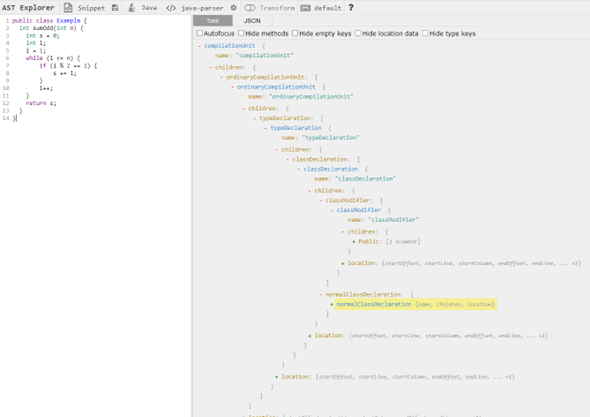
\includegraphics [scale=0.27] {my_folder/images/my/9}
	\caption{Результат работы AST Explorer} 
	\label{fig:9}  
\end{figure}
%\section{VisualDFA} \label{ch2:sec1-abbr}
\subsection{VisualDFA} \label{ch2:subsec-title-abbr}
VisualDFA – это сложный образовательный инструмент для визуализации анализа потоков данных с использованием Java/Jimple, который позволяет:
\begin{itemize}
\item Запускать 4 встроенных анализа: сворачивание констант (Constant Folding), биты констант (Constant Bits), достигающие определения (Reaching Definitions) и проверка на заражённость (Taint Analysis)
\item Вводить Java-код, либо подключать его из файла
\item Визуализировать код с помощью CFG
\item Выполнять код пошагово, либо продолжить до следующей установленной точки остановки
\item Видеть входные и выходные данные для любого блока или строки кода в любой момент времени
\item Экспорт CFG в PNG-файл или вывод одной командой изображений всех шагов анализа
\item Внедрять и запускать пользовательские анализы без перекомпиляции VisualDFA
\end{itemize}
Этот инструмент строит CFG в интерфейсе своего приложения. Внешний вид получаемого CFG не такой, как хотелось бы его видеть. У каждого блока вверху есть пустая область, за которую блок можно перетаскивать. При этом во время перетаскивания размещение стрелок происходит странным образом. Они пересекают другие блоки и частично остаются на начальных позициях. Так же блоки начала метода, условий и обычных операторов визуально не отличаются. От условий идут стрелки, смотря на которые непонятно, по какой из них переходить в случае, если условие истинно, и по какой в случае, если ложно. Создаются временные переменные там, где их нет в коде. Почему-то сами условия записываются противоположно тем, которые написаны в коде.
Как итог, VisualDFA можно назвать готовым решением для построения и визуализации CFG, но результат оставляет желать лучшего.
\begin{figure}[ht!] 
	\center
	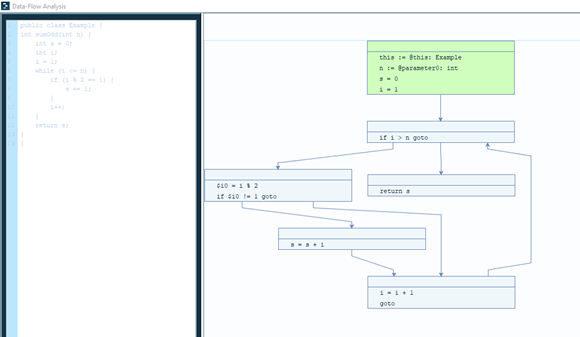
\includegraphics [scale=0.27] {my_folder/images/my/10}
	\caption{Результат работы VisualDFA} 
	\label{fig:10}  
\end{figure}
\subsection{VisualControlFlowGraph4J} \label{ch2:subsec-title-abbr}
VisualControlFlowGraph4J – инструмент для построения и визуализации Java-кода в виде CFG, использующий ANTLR и GraphViz.
Инструмент помогает строить CFG, но у него также есть ряд недостатков. Построение CFG нельзя назвать интерактивным. Он требует файла с исходным кодом в папке с ресурсами для того, чтобы строить модель по нему. Граф сохраняется в файловую систему в виде SVG-файла по завершению работы программы. В самом CFG присутствуют обозначения типов данных, что делает граф привязанным к языку программирования. Также наблюдается проблема с тем, что, смотря на стрелки, исходящие из блоков условий, непонятно, по какой из них переходить при истинном или ложном условии. Кроме того, никак не обозначены параметры метода, граф для которого строится.
VisualControlFlowGraph4J можно считать готовым решением для построения и визуализации CFG, но не лишённым своих недостатков.
\begin{figure}[ht!] 
	\center
	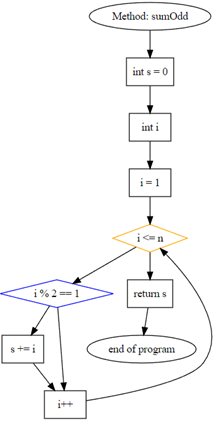
\includegraphics [scale=0.27] {my_folder/images/my/11}
	\caption{Результат работы VisualControlFlowGraph4J} 
	\label{fig:11}  
\end{figure}
\section{Выводы по главе} \label{ch2:sec2}
В данной главе проведен обзор и анализ существующих средств визуализации моделей программ. Были найдены лишь решения для AST и CFG, для визуализации остальных моделей программ не было найдено ни одного достойного решения. Также хочется отметить, что не существует ни одного сервиса, способного интерактивно визуализировать несколько разных моделей программ. На основе результата обзора можно сделать вывод о том, что тема выпускной квалификационной работы является актуальной.
\newpage











% не рекомендуется использовать отдельную section <<введение>> после лета 2020 года
%\section{Введение} \label{ch2:intro}

%Глава посвящена более подробным примерам оформления текстово-графических объектов.
%
%В параграфе \ref{ch2:title-abbr} приведены примеры оформления многострочной формулы и одиночного рисунка. Параграф \ref{ch2:sec-abbr} раскрывает правила оформления перечислений и псевдокода. В параграфе \ref{ch2:sec-very-short-title} приведены примеры оформления сложносоставных рисунков, длинных таблиц, а также теоремоподобных окружений.
%
%
%\section{Название параграфа} \label{ch2:title-abbr} %название по-русски
%
%
%
%%%%%
%%%		
%%%  \input{...} commands are used only to sychronize some parts of the text with the author guide. Authors are free to type the text directly in .tex-files   
%%%  \input{...} комманды используются только, чтобы синхронизировать части текта с рекомендациями авторам. Авторы  вольны вносить текст непосредственно в файл главы  
%%%  
% \input{my_folder/tex/eq-Galois} % пример двух выравнивания двух формул в окружении align
%
%
%На \firef{fig:spbpu-new-bld-autumn-ch2} приведёна фотография Нового научно-исследовательского корпуса СПбПУ.
%
%	\begin{figure}[ht] 
%	\center
%	\includegraphics [scale=0.27] {my_folder/images/spbpu_new_bld_autumn}
%	\caption{Новый научно-исследовательский корпус СПбПУ \cite{spbpu-gallery}} 
%	\label{fig:spbpu-new-bld-autumn-ch2}  
%	\end{figure}
%	
%
%
%	
%\section{Название параграфа} \label{ch2:sec-abbr} %название по-русски
%	
%Название параграфа оформляется с помощью команды \verb|\section{...}|, название главы --- \verb|\chapter{...}|. 
%	
%
%\subsection{Название подпараграфа} \label{ch2:subsec-title-abbr} %название по-русски
%
%
%Название подпараграфа оформляется с помощью команды  \texttt{\textbackslash{}subsection\{...\}}.
%
%
%%\subsubsection{Название подподпараграфа} \label{ch2:subsubsec-title-abbr} %название по-русски
%	
%Использование подподпараграфов в основной части крайне не рекомендуется. В случае использования, необходимо вынести данный номер в содержание.	
%Название подпараграфа оформляется с помощью команды  \texttt{\textbackslash{}subsubsecti\-on\{...\}}.
%
%
%
%\input{my_folder/tex/enumeration} % правила использования перечислений	
%
%	
%Оформление псевдокода необходимо осуществлять с помощью пакета \verb|algorithm2e| в окружении \verb|algorithm|. Данное окружение интерпретируется в шаблоне как рисунок. Пример оформления псевдокода алгоритма приведён на \firef{alg:AlgoFDSCALING}. 
%	
%	
%\input{my_folder/tex/pseudocode-agl-DTestsFDScaling} % пример оформления псевдокода алгоритма 	
%
%	
%\section{Название параграфа} \label{ch2:sec-very-short-title} %название по-русски
%
%
%	
%\input{my_folder/tex/eq-equation-multilined} % пример оформления одиночной формулы в несколько строк
%
%\input{my_folder/tex/fig-spbpu-sc-four-in-one} % пример подключения 4х иллюстраций в одном рисунке
%
%%\input{my_folder/tex/fig-spbpu-whitehall-three-in-one} % пример подключения 3х иллюстрации в одном рисунке
%%
%%\input{my_folder/tex/fig-spbpu-main-bld-two-in-one} % пример подключения 2х иллюстраций в одном рисунке
%
%\input{my_folder/tex/tab-more-than-one-page} % пример подключения таблицы на несколько страциц
%
%
%\begin{table} [htbp]% Пример оформления таблицы
%	\centering\small
%	\caption{Пример представления данных для сквозного примера по ВКР \cite{Peskov2004}}%
%	\label{tab:ToyCompare}		
%		\begin{tabular}{|l|l|l|l|l|l|}
%			\hline
%			$G$&$m_1$&$m_2$&$m_3$&$m_4$&$K$\\
%			\hline
%			$g_1$&0&1&1&0&1\\ \hline
%			$g_2$&1&2&0&1&1\\ \hline
%			$g_3$&0&1&0&1&1\\ \hline
%			$g_4$&1&2&1&0&2\\ \hline
%			$g_5$&1&1&0&1&2\\ \hline
%			$g_6$&1&1&1&2&2\\ \hline		
%		\end{tabular}
%%	\caption*{\raggedright\hspace*{2.5em} Составлено (или/и рассчитано) по \cite{Peskov2004}} %Если проведена авторская обработка или расчеты по какому-либо источнику	
%	\normalsize% возвращаем шрифт к нормальному
%\end{table}
%
%
%
%%% please, before using, read the author guide carefully
%
%\input{my_folder/tex/tab-toy-context-minipage} % пример подключения minipage
%
%\input{my_folder/tex/fig-spbpu-new-bld-autumn-minipage} % пример подключения minipage
%
%
%
%
%\input{my_folder/tex/rules-theorem-like-expressions} 
%
%По аналогии с нумерацией формул, рисунков и таблиц нумеруются и иные текстово-графические объекты, то есть включаем в нумерацию номер главы, например: теорема 3.1. для первой теоремы третьей главы монографии. Команды \LaTeX{} выставляют нумерацию и форматирование автоматически. Полный перечень команд для подготовки текстово-графических и иных объектов находится в подробных методических рекомендациях \cite{spbpu-bci-template-author-guide}. 
%
%
%\input{my_folder/tex/rules-list-of-environments} % список некоторых окружений
%
%
%\input{my_folder/tex/theorem-example} %пример оформления теоремы
%
%
%\input{my_folder/tex/definition-example} %пример оформления определения
%
%
%Вместо теоремо-подобных окружений для вставки небольших текстово-графических объектов иногда используются команды. Типичным примером такого подхода является команда \verb|\footnote{text}|\footnote{Внимание! Команда вставляется непосредственно после слова, куда вставляется сноска (без пробела). Лишние пробелы также не указываются внутри команды перед и после фигурных скобок.}, где в аргументе \verb|text| указывают текст \textit{подстрочной ссылки (сноски)}.В них \textit{нельзя добавлять веб-ссылки или цитировать литературу}. Для этих целей используется список литературы. Нумерация сносок сквозная по ВКР без точки на конце выставляется в шаблоне автоматически, однако в каждом приложении к ВКР нумерация, зависящая от номера приложения, выставляется префикс <<П>>, например <<П1.1>> --- первая сноска первого приложения. 
%
%
%
%
%%\FloatBarrier % заставить рисунки и другие подвижные (float) элементы остановиться
%
%
%\section{Выводы} \label{ch2:conclusion}
%
%Текст заключения ко второй главе. Пример ссылок \cite{Article,Book,Booklet,Conference,Inbook,Incollection,Manual,Mastersthesis,Misc,Phdthesis,Proceedings,Techreport,Unpublished,badiou:briefings}, а также ссылок с указанием страниц, на котором отображены те или иные текстово-графические объекты  \cite[с.~96]{Naidenova2017} или в виде мультицитаты на несколько источников \cites[с.~96]{Naidenova2017}[с.~46]{Ganter1999}. Часть библиографических записей носит иллюстративный характер и не имеет отношения к реальной литературе. 
%
%Короткое имя каждого библиографического источника содержится в специальном файле \verb|my_biblio.bib|, расположенном в папке \verb|my_folder|. Там же находятся исходные данные, которые с помощью программы \texttt{Biber} и стилевого файла \texttt{Biblatex-GOST} \cite{ctan-biblatex-gost} приведены в списке использованных источников согласно ГОСТ 7.0.5-2008.
%Многообразные реальные примеры исходных библиографических данных можно посмотреть по ссылке \cite{ctan-biblatex-gost-examples}.
%
%Как правило, ВКР должна состоять из четырех глав. Оставшиеся главы можно создать по образцу первых двух и подключить с помощью команды \verb|\input| к исходному коду ВКР. Далее в приложении \ref{appendix-MikTeX-TexStudio} приведены краткие инструкции запуска исходного кода ВКР \cite{latex-miktex,latex-texstudio}.
%
%В приложении \ref{appendix-extra-examples} приведено подключение некоторых текстово-графических объектов. Они оформляются по приведенным ранее правилам. В качестве номера структурного элемента вместо номера главы используется <<П>> с номером главы. Текстово-графические объекты из приложений не учитываются в реферате.
%
%
%
%%% Вспомогательные команды - Additional commands
%%
%%\newpage % принудительное начало с новой страницы, использовать только в конце раздела
%%\clearpage % осуществляется пакетом <<placeins>> в пределах секций
%%\newpage\leavevmode\thispagestyle{empty}\newpage % 100 % начало новой страницы